%%%%%%%%%%%%%%%%%%%%%%%%%%%%%%%%%%%%%%%%%%%%%%%%%%%%%%%%%%%%%%%%%%
%%%%%%%%%%%%%%%%%%%%%%%%%%%%%%%%%%%%%%%%%%%%%%%%%%%%%%%%%%%%%%%%%%

\subsection{Compilation}
Quand on veut compiler un simple code C en utilisant \acrshort{gcc} par
exemple, le compilateur passe par plusieurs étapes. Le préprocesseur génère d'abord
un fichier C en fonction des directives de préprocesseur. Ce fichier C est ensuite
compilé en code assembleur qui est lui même compilé en code objet. Le \textit{linker}
permet ensuite de lier les différents fichiers objets et générer un exécutable.
Nous avons déjà eu un aperçu des différentes étapes de la compilation d'un \acrshort{os}
de type \textit{bare metal} dans la partie \ref{technologies}. A la différence de
la compilation d'un code C, nous avons d'un côté du code assembleur et de l'autre
du code Rust. Nasm et cargo permettent tous deux de générer des fichiers objets.
Il n'y a donc que la dernière étape à effectuer ce que \acrshort{gcc} permet de
faire avec la commande suivante.
\begin{minted}[tabsize=4]{shell}
gcc $(OBJS) -T $(LINKER) -static -m32 -ffreestanding -nostdlib -o $@ $(RUST)
\end{minted}
Ici, \mintinline{shell}{$(OBJS)} représente les fichiers objets générés par
\mintinline{rust}{nasm}, \mintinline{shell}{$(LINKER)} est un fichier permettant
de faire l'édition des liens et \mintinline{shell}{$(RUST)} représente les fichiers
objets générés par Rust.\cite{ref42}

%%%%%%%%%%%%%%%%%%%%%%%%%%%%%%%%%%%%%%%%%%%%%%%%%%%%%%%%%%%%%%%%%%
%%%%%%%%%%%%%%%%%%%%%%%%%%%%%%%%%%%%%%%%%%%%%%%%%%%%%%%%%%%%%%%%%%

\subsection{\textit{Linking}}
\label{linking}
Nous avons vu dans la partie précédente que \acrshort{gcc} a besoin d'un fichier
pour faire l'édition des liens. Si ce fichier n'est pas donné, il en utilise un par
défaut. Le \textit{linker} permet de structurer le code par sections. Prenons
pour exemple le \textit{script} utilisé pour ce projet.

\begin{minted}[fontsize=\footnotesize,linenos,frame=single,tabsize=4]{c}
ENTRY(entrypoint)
SECTIONS {
  . = 1M;
  .boot ALIGN(4):
  {
    *(.multiboot)
  }
  .stack ALIGN(4):
  {
    *(.stack)
  }
  .text ALIGN(4K) :
  {
    *(.text*)
  }
  .rodata ALIGN(4K) :
  {
    *(.rodata*)
  }
  .data ALIGN(4K) :
  {
    *(.data*)
  }
  .bss ALIGN(4K) :
  {
    *(COMMON)
    *(.bss*)
  }
}
\end{minted}

L'appel à \mintinline{c}{ENTRY} permet de spécifier l'entrée du \textit{kernel}.
Pour un simple programme en C l'entrée serait le \textit{main}. Ici, ce sera
l'entrée de notre \textit{kernel} donc la première fonction exécutée au \textit{boot}.
\mintinline{text}{SECTION} va dire au linker où placer les parties du code. Par exemple, 
la section \mintinline{text}{.text} contiendra le code et la section \mintinline{text}{.data}
contiendra les variables initialisées \cite{ref42,ref9,ref10,ref11}. Voici donc la structure
du fichier \acrshort{elf} qui serait généré à l'aide de ce \textit{script}.

\begin{figure}[!h]
  \centering
  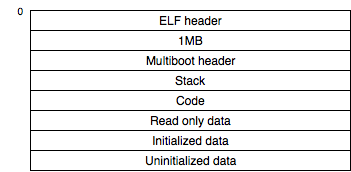
\includegraphics[scale=0.75]{images/elf_struct.png}
  \caption{Strucutre du fichier \acrshort{elf}}
\end{figure}

A noter que les sections commencent avec un \textit{offset} de 1MB. Nous avons eu
besoin de faire ça car les premiers 1MB dans un \acrshort{os} sont reservés \cite{ref42,ref13}.
La mémoire vidéo (\acrshort{vram}) se situe par exemple dans cette zone.

%%%%%%%%%%%%%%%%%%%%%%%%%%%%%%%%%%%%%%%%%%%%%%%%%%%%%%%%%%%%%%%%%%
%%%%%%%%%%%%%%%%%%%%%%%%%%%%%%%%%%%%%%%%%%%%%%%%%%%%%%%%%%%%%%%%%%

\subsection{\textit{Boot}}
\subsubsection{Principe général}
Quand un ordinateur est allumé, un signal est envoyé à la carte mère qui démarre
l'alimentation. Le processeur démarre alors en mode 16-bits. Le signal "Power Ok"
est envoyé au \acrshort{bios} qui est le \textit{firmware} du \acrshort{pc}
(localisé en mémoire flash de la carte mère). Le \acrshort{bios} initialise alors
la séquence POST (\textit{Power On Self Test}) qui vérifie que chaque périphérique
est alimenté et que la mémoire est ok puis initialise chaque périphérique et enfin
redonne la main au \acrshort{bios} qui continue le \textit{boot}. Le \acrshort{bios}
charge ensuite les 512 premiers bytes (\acrshort{mbr}) du premier disque qui doit
charger le \textit{kernel} en mémoire et l'exécuter. Pour résumer, le \textit{boot}
d'une machine à base de \acrshort{bios} se déroule de la manière ci-dessous.\cite{ref42}

\begin{figure}[!h]
  \centering
  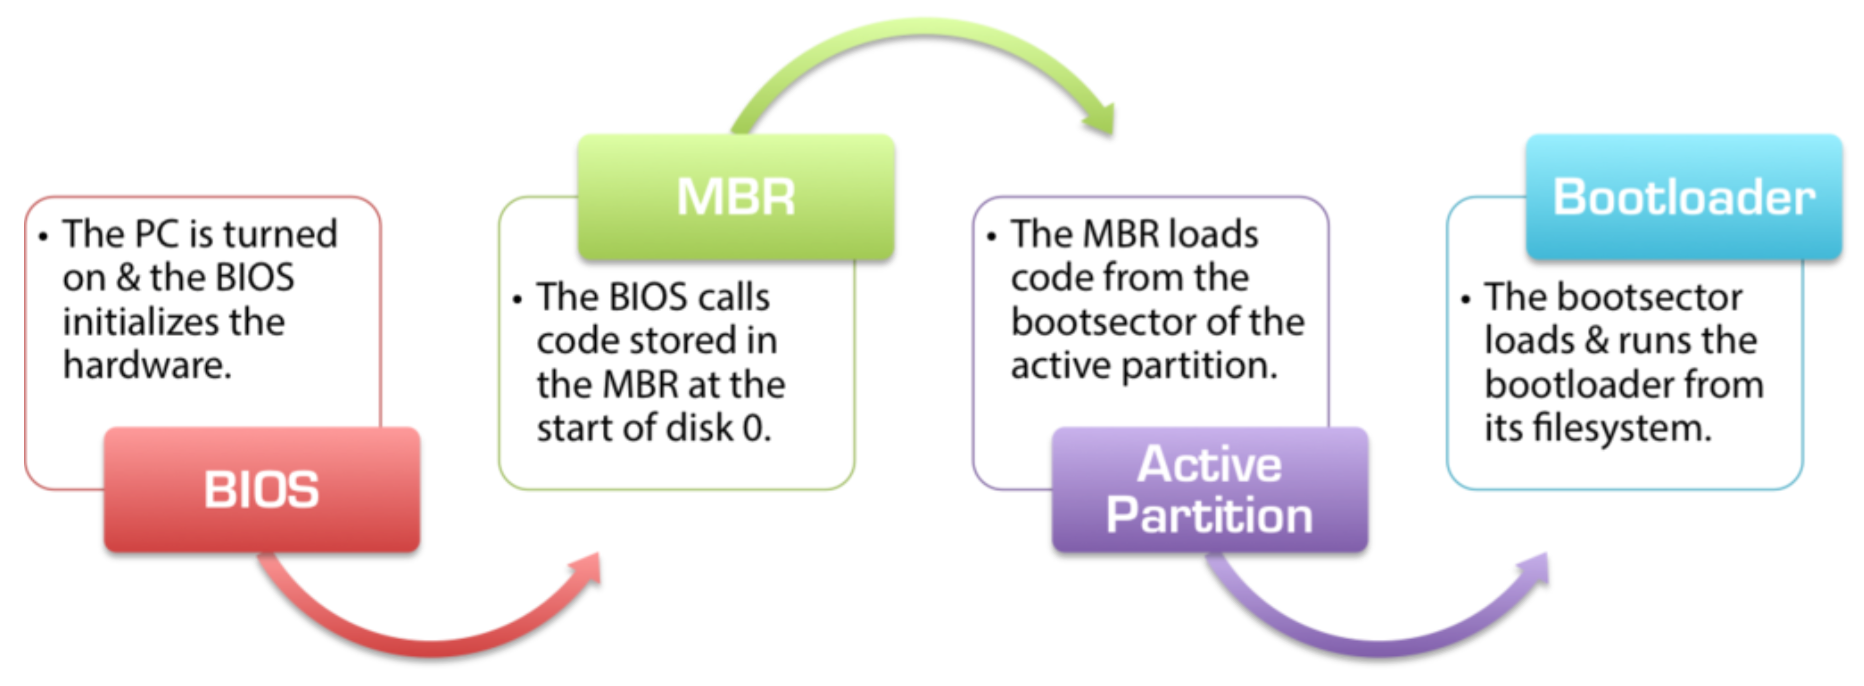
\includegraphics[scale=0.4]{images/bios_boot.png}
  \caption{\textit{Boot} d'une machine à base de \acrshort{bios}}
\end{figure}

%%%%%%%%%%%%%%%%%%%%%%%%%%%%%%%%%%%%%%%%%%%%%%%%%%%%%%%%%%%%%%%%%%

\subsubsection{\acrshort{grub}}
Le \acrshort{mbr} contient ce qui est appelé le \textit{bootloader}. Le \textit{bootloader}
est le morceau de code qui va charger le \textit{kernel} en mémoire et l'exécuter.
C'est ici qu'entre en scène \acrshort{grub}. \acrshort{grub} est un \textit{bootloader}
puissant et versatile permettant de charger n’importe quel type de système d’exploitation.
Son initialisation se fait par étapes.
\begin{itemize}[label=\textbullet]
	\item \textit{Stage} 1: Chargé en mémoire par le \acrshort{bios} depuis le
    \acrshort{mbr}, il contient le code pour charger le \textit{Stage} 1.5
	\item \textit{Stage} 1.5: Chargé en mémoire par le \textit{Stage} 1, il contient
    les drivers nécessaires à l'accès au système de fichiers par le \textit{Stage} 2
	\item \textit{Stage} 2: Chargé en mémoire par le \textit{Stage} 1.5, il affiche
    le menu de \acrshort{grub}. Il permet de sélectionner et charger un \acrshort{os}
\end{itemize}

\acrshort{grub} permet de charger n'importe quel type de système d'exploitation
grace au standard \textit{Multiboot}. Ce standard permet à tout \textit{bootloader}
de charger tout \acrshort{os} compatible \cite{ref42,ref12}.

\subsubsection{Image \acrshort{iso}}
Nous avons déjà pu voir que le \textit{boot} du \textit{kernel} se faisait à partie
d'une image \acrshort{iso} dans la partie \ref{qemu}. Pour qu'une image \acrshort{iso}
soit \textit{bootable}, il est nécessaire que \acrshort{grub} soit installé dans
les huit premiers KB du disque. Prenons l'arborescence suivante :

\begin{minted}[tabsize=4]{shell}
isofiles
└── boot
    └── grub
\end{minted}

Les fichiers \mintinline{text}{kernel.elf} (kernel sur lequel nous voulons
\textit{booter}), \mintinline{text}{menu.lst} (fichier de configuration de \acrshort{grub})
et \mintinline{text}{stage2_eltorito} doivent être copiés de manière à obtenir
l'arborescence suivante :

\begin{minted}[tabsize=4]{text}
isofiles
└── boot
    ├── grub
    │   ├── menu.lst
    │   └── stage2_eltorito
    └── kernel.elf
\end{minted}

Pour finir, il faut exécuter la commande :
\begin{minted}[tabsize=4]{shell}
genisoimage -R -b boot/grub/stage2_eltorito -input-charset utf8 -no-emul-boot \
-boot-info-table -o os.iso isofiles
\end{minted}
Cette commande génerera une image \acrshort{iso} \textit{bootable} nommée \mintinline{text}{os.iso}\cite{ref42}.